% Communication over a noisy channel (notebook 50, Section 1 and Figure 1): a source emits k message bits with entropy
% H(X); the encoder adds redundancy and sends n >= k bits (rate R = k/n); the binary symmetric channel flips each bit
% with probability q; the decoder uses the redundancy to correct errors; the receiver gets an estimate of the message.
% Example: the Hamming(7,4) code of Section 6.2, message 1011 -> codeword 0110011, one error at position 5.
% Information quantities: H(X) at the source, I(X:Y) = H(X) - H(X|Y) per channel use, capacity C = 1 - h(q).
\documentclass[tikz,border=6pt]{standalone}
\usepackage{amsmath,amssymb}
\usetikzlibrary{arrows.meta,positioning,calc,decorations.pathreplacing}
\begin{document}
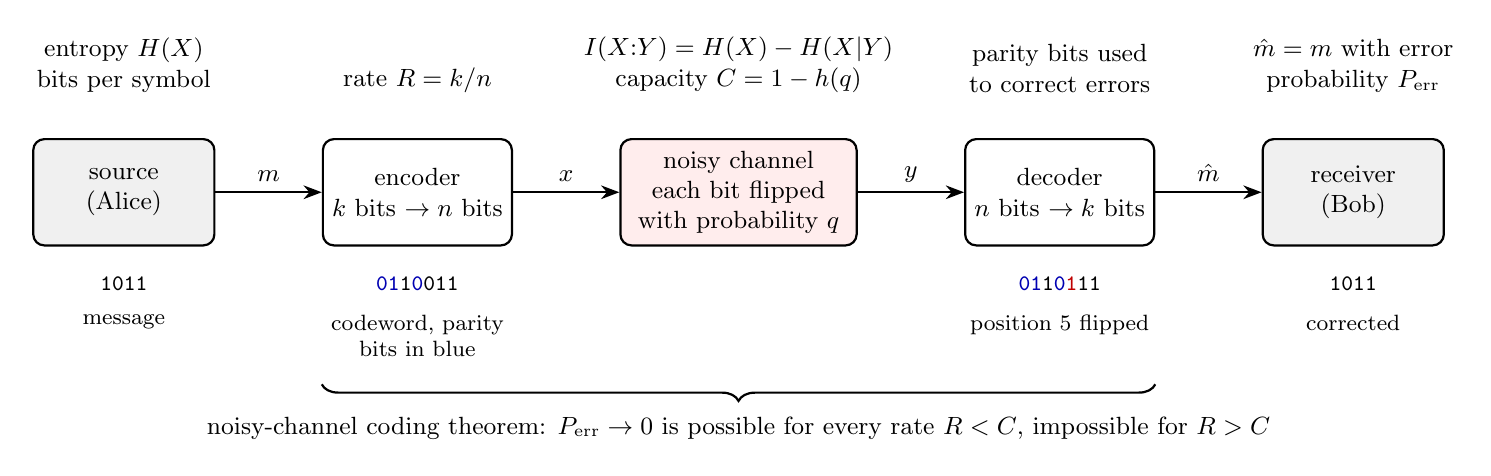
\begin{tikzpicture}[thick, >=Stealth, node distance=1.35cm,
    box/.style={draw, rounded corners, fill=white, minimum height=1.35cm, minimum width=2.3cm, align=center, font=\small},
    noisy/.style={box, fill=red!7}]
  \node[box, fill=black!6] (src) {source\\ (Alice)};
  \node[box, right=of src] (enc) {encoder\\ $k$ bits $\to n$ bits};
  \node[noisy, right=of enc, minimum width=3.0cm] (ch) {noisy channel\\ each bit flipped\\ with probability $q$};
  \node[box, right=of ch] (dec) {decoder\\ $n$ bits $\to k$ bits};
  \node[box, fill=black!6, right=of dec] (rcv) {receiver\\ (Bob)};
  \draw[->] (src) -- node[above, font=\small] {$m$} (enc);
  \draw[->] (enc) -- node[above, font=\small] {$x$} (ch);
  \draw[->] (ch) -- node[above, font=\small] {$y$} (dec);
  \draw[->] (dec) -- node[above, font=\small] {$\hat m$} (rcv);
  % example strings: Hamming(7,4) of Section 6.2, message 1011 -> codeword 0110011 (check positions 1, 2, 4 in blue)
  \newcommand{\pb}[1]{\textcolor{blue!70!black}{\texttt{#1}}}
  \node[font=\footnotesize\ttfamily, below=0.25cm of src] (ms) {1011};
  \node[font=\footnotesize\ttfamily, below=0.25cm of enc] (xs) {\pb{01}1\pb{0}011};
  \node[font=\footnotesize\ttfamily, below=0.25cm of dec] (ys) {\pb{01}1\pb{0}\textcolor{red!75!black}{\texttt{1}}11};
  \node[font=\footnotesize\ttfamily, below=0.25cm of rcv] (mh) {1011};
  \node[font=\footnotesize, align=center, below=0.05cm of ms] {message};
  \node[font=\footnotesize, align=center, below=0.05cm of xs] {codeword, parity\\ bits in blue};
  \node[font=\footnotesize, align=center, below=0.05cm of ys] {position 5 flipped};
  \node[font=\footnotesize, align=center, below=0.05cm of mh] {corrected};
  % information quantities
  \node[font=\small, align=center, above=0.45cm of src] {entropy $H(X)$\\ bits per symbol};
  \node[font=\small, align=center, above=0.45cm of enc] {rate $R=k/n$};
  \node[font=\small, align=center, above=0.45cm of ch] {$I(X{:}Y)=H(X)-H(X\vert Y)$\\ capacity $C=1-h(q)$};
  \node[font=\small, align=center, above=0.45cm of dec] {parity bits used\\ to correct errors};
  \node[font=\small, align=center, above=0.45cm of rcv] {$\hat m=m$ with error\\ probability $P_{\rm err}$};
  % theorem bracket
  \draw[decorate, decoration={brace, amplitude=6pt, mirror}] ($(enc.south west)+(0,-1.75)$) -- ($(dec.south east)+(0,-1.75)$)
       node[midway, below=8pt, font=\small] {noisy-channel coding theorem: $P_{\rm err}\to0$ is possible for every rate $R<C$, impossible for $R>C$};
\end{tikzpicture}
\end{document}
